\section{Versuchsaufbau}

\subsection{Aufbau zur Messung der \textgamma-Spektren von \texorpdfstring{${}^{22}$Na, ${}^{60}$Co, ${}^{152}$Eu und ${}^{228}$Th}{22-Na, 60-Co, 152-Eu und 228-Th}.}

\begin{figure}[H]
\begin{center}
  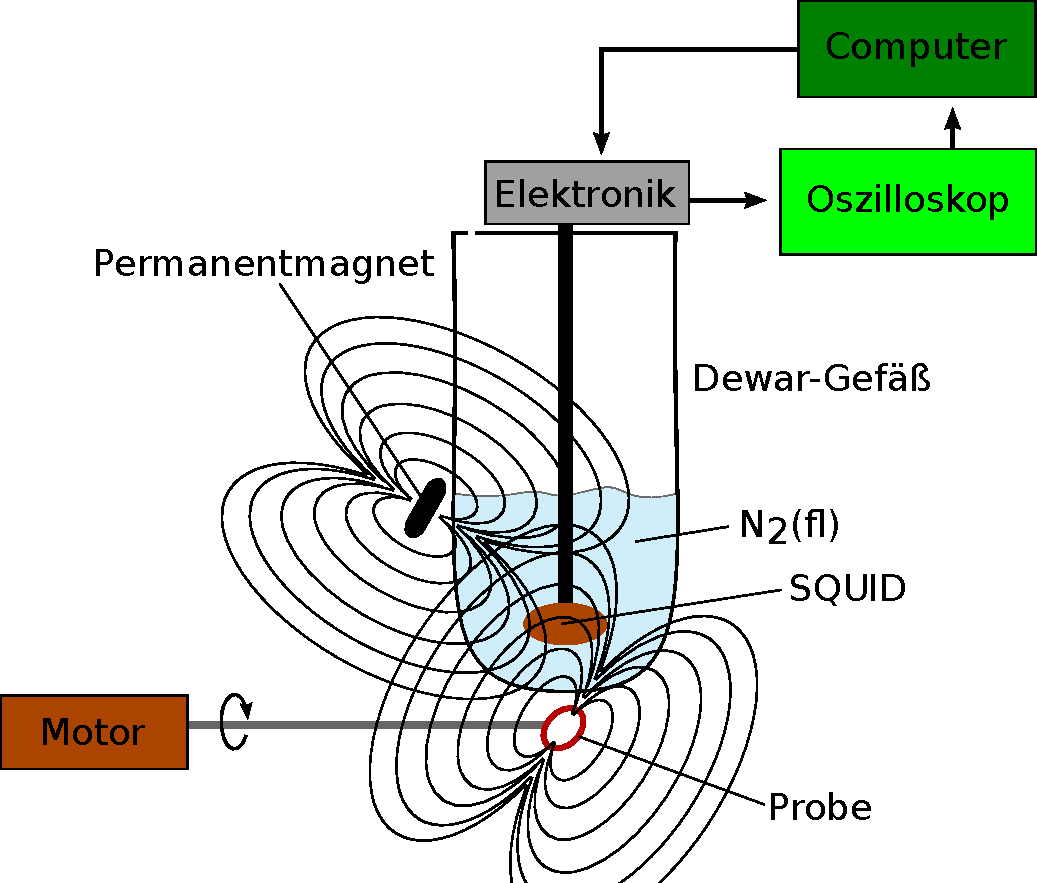
\includegraphics[width=\textwidth]{../img/aufbau.pdf}
  \caption[---]{Aufbau zur Energiebestimmung von \textgamma-Strahlung.}
  \label{img:aufbau}
\end{center}
\end{figure}

\autoref{img:aufbau} zeigt den Aufbau, wie er für die Messung der \textgamma-Spektren verwendet wird:
Die hochenergetische Strahlung aus den radioaktiven Präparaten fällt auf einen NaJ-Kristall und
erzeugt dort Photonen im sichtbaren Bereich, die von einem Photomultiplier registriert werden.
Die Spannungsversorgung für den Photomultiplier erfolgt über ein Netzteil (HV).
Im Gehäuse des Photomultipliers ist zusätzlich ein Vorverstärker untergebracht.
Vom Vorverstärker gelangt das Signal in den Hauptverstärker und aus dessen unipolarem Ausgang
in den \emph{multi-channel-analyser}.
Die Messdaten des MCAs werden mit dem Computer aufgenommen.


\subsection{Aufbau zur Koinzidenzmessung}

\begin{figure}[H]
\begin{center}
  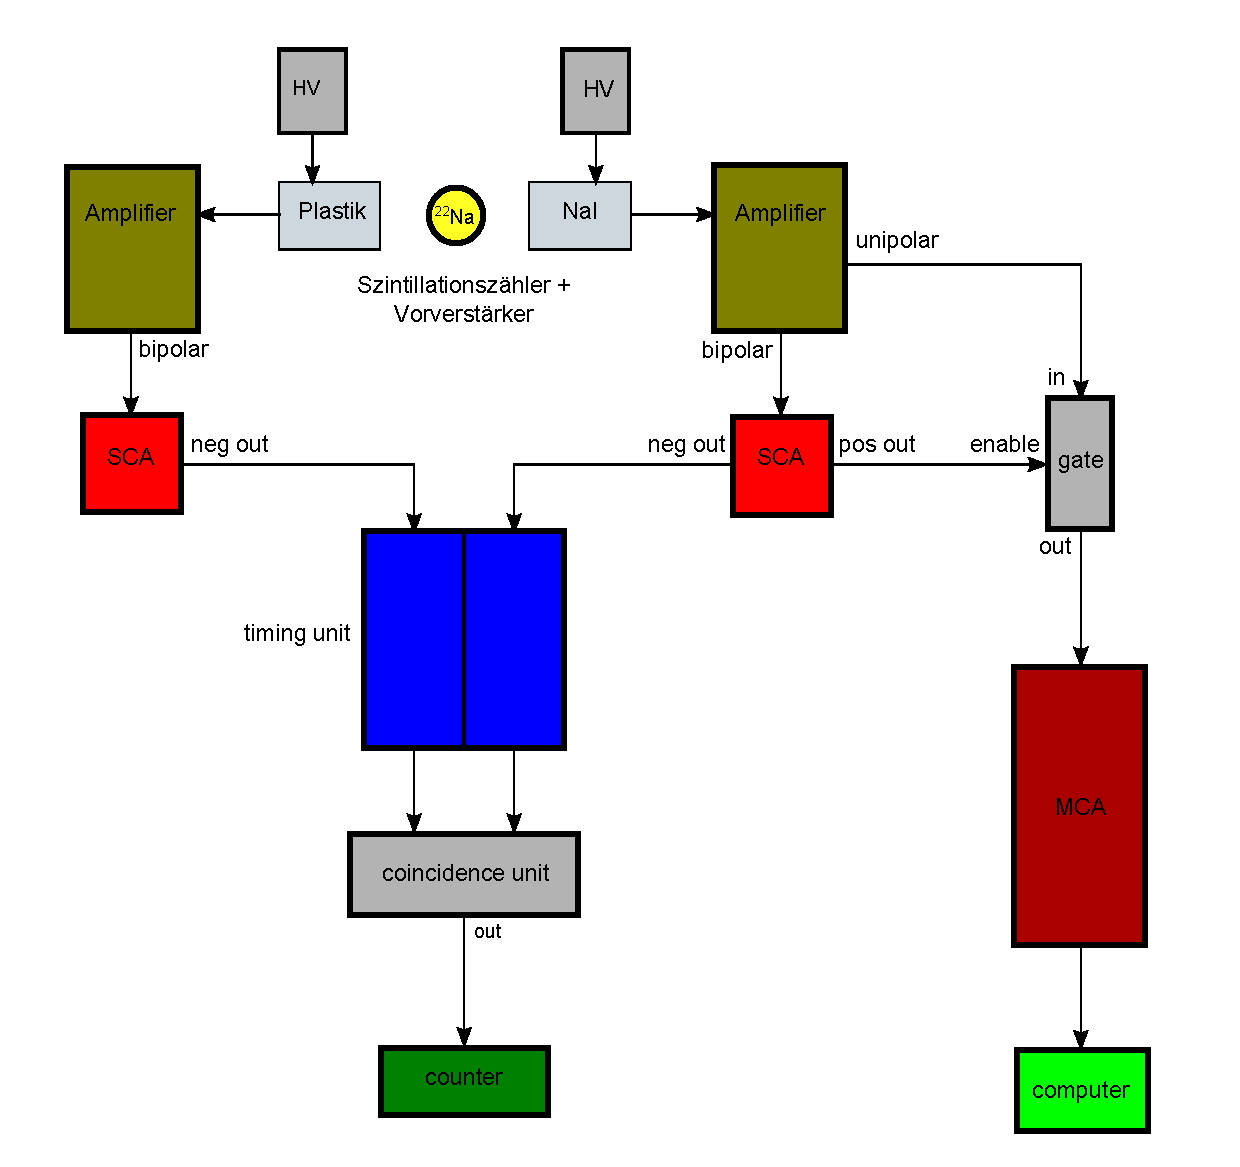
\includegraphics[width=\textwidth]{../img/aufbau2.pdf}
  \caption[---]{Aufbau zur Messung von koinzidierenden Vernichtungsphotonen
  des $\beta^-$Zerfalls von ${}^{22}$Na}
  \label{img:aufbau2}
\end{center}
\end{figure}

%TODO Winkelgeschichte beschreiben

Auf \autoref{img:aufbau2} ist der komplexere Aufbau für die Messung von Koinzidenzen gezeigt.
Es werden sowohl der Plastik- als auch der NaJ-Szintillator verwendet, deren Ausgangssignale
verstärkt werden.
Das bipolare Ausgangssignal der Verstärker gelangt in zwei \emph{single channel analyser},
dann in zwei verschiedene Kanäle einer \emph{timing unit} und schließlich in eine Koinzidenzeinheit,
die im Falle einer Koinzidenz ein Signal an einen Zähler gibt.
Der unipolare Ausgang des Verstärkers nach dem NaJ-Kristall wird wie in \autoref{img:aufbau}
für die Energiemessung mit dem MCA verbunden. Vor dem MCA befindet sich allerdings eine Weiche,
die vom SCA gesteuert wird und daher nur Signale mit geeigneter Amplitude passieren lässt.
Auf die Funktionsweise der einzelnen Geräte, ihren Anschluss und die Einstellparameter
wird im nächsten Abschnitt genauer eingegangen.



